% !TEX encoding = UTF-8 Unicode
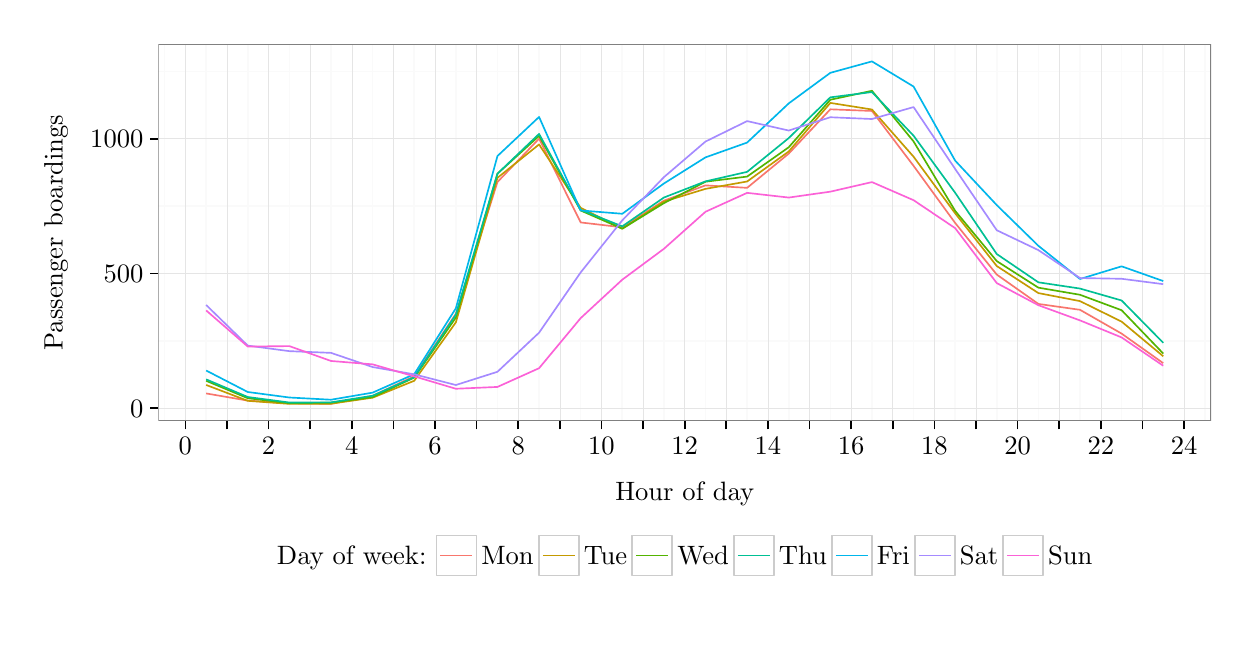
\begin{tikzpicture}[x=1pt,y=1pt]
\definecolor{fillColor}{RGB}{255,255,255}
\path[use as bounding box,fill=fillColor,fill opacity=0.00] (0,0) rectangle (433.62,216.81);
\begin{scope}
\path[clip] (  0.00,  0.00) rectangle (433.62,216.81);
\definecolor{drawColor}{RGB}{255,255,255}
\definecolor{fillColor}{RGB}{255,255,255}

\path[draw=drawColor,line width= 0.6pt,line join=round,line cap=round,fill=fillColor] (  0.00,  0.00) rectangle (433.62,216.81);
\end{scope}
\begin{scope}
\path[clip] ( 47.21, 74.69) rectangle (427.62,210.81);
\definecolor{fillColor}{RGB}{255,255,255}

\path[fill=fillColor] ( 47.21, 74.69) rectangle (427.62,210.81);
\definecolor{drawColor}{gray}{0.98}

\path[draw=drawColor,line width= 0.6pt,line join=round] ( 47.21,103.64) --
	(427.62,103.64);

\path[draw=drawColor,line width= 0.6pt,line join=round] ( 47.21,152.33) --
	(427.62,152.33);

\path[draw=drawColor,line width= 0.6pt,line join=round] ( 47.21,201.01) --
	(427.62,201.01);

\path[draw=drawColor,line width= 0.6pt,line join=round] ( 49.46, 74.69) --
	( 49.46,210.81);

\path[draw=drawColor,line width= 0.6pt,line join=round] ( 64.50, 74.69) --
	( 64.50,210.81);

\path[draw=drawColor,line width= 0.6pt,line join=round] ( 79.53, 74.69) --
	( 79.53,210.81);

\path[draw=drawColor,line width= 0.6pt,line join=round] ( 94.57, 74.69) --
	( 94.57,210.81);

\path[draw=drawColor,line width= 0.6pt,line join=round] (109.61, 74.69) --
	(109.61,210.81);

\path[draw=drawColor,line width= 0.6pt,line join=round] (124.64, 74.69) --
	(124.64,210.81);

\path[draw=drawColor,line width= 0.6pt,line join=round] (139.68, 74.69) --
	(139.68,210.81);

\path[draw=drawColor,line width= 0.6pt,line join=round] (154.72, 74.69) --
	(154.72,210.81);

\path[draw=drawColor,line width= 0.6pt,line join=round] (169.75, 74.69) --
	(169.75,210.81);

\path[draw=drawColor,line width= 0.6pt,line join=round] (184.79, 74.69) --
	(184.79,210.81);

\path[draw=drawColor,line width= 0.6pt,line join=round] (199.82, 74.69) --
	(199.82,210.81);

\path[draw=drawColor,line width= 0.6pt,line join=round] (214.86, 74.69) --
	(214.86,210.81);

\path[draw=drawColor,line width= 0.6pt,line join=round] (229.90, 74.69) --
	(229.90,210.81);

\path[draw=drawColor,line width= 0.6pt,line join=round] (244.93, 74.69) --
	(244.93,210.81);

\path[draw=drawColor,line width= 0.6pt,line join=round] (259.97, 74.69) --
	(259.97,210.81);

\path[draw=drawColor,line width= 0.6pt,line join=round] (275.00, 74.69) --
	(275.00,210.81);

\path[draw=drawColor,line width= 0.6pt,line join=round] (290.04, 74.69) --
	(290.04,210.81);

\path[draw=drawColor,line width= 0.6pt,line join=round] (305.08, 74.69) --
	(305.08,210.81);

\path[draw=drawColor,line width= 0.6pt,line join=round] (320.11, 74.69) --
	(320.11,210.81);

\path[draw=drawColor,line width= 0.6pt,line join=round] (335.15, 74.69) --
	(335.15,210.81);

\path[draw=drawColor,line width= 0.6pt,line join=round] (350.18, 74.69) --
	(350.18,210.81);

\path[draw=drawColor,line width= 0.6pt,line join=round] (365.22, 74.69) --
	(365.22,210.81);

\path[draw=drawColor,line width= 0.6pt,line join=round] (380.26, 74.69) --
	(380.26,210.81);

\path[draw=drawColor,line width= 0.6pt,line join=round] (395.29, 74.69) --
	(395.29,210.81);

\path[draw=drawColor,line width= 0.6pt,line join=round] (410.33, 74.69) --
	(410.33,210.81);

\path[draw=drawColor,line width= 0.6pt,line join=round] (425.36, 74.69) --
	(425.36,210.81);
\definecolor{drawColor}{gray}{0.90}

\path[draw=drawColor,line width= 0.2pt,line join=round] ( 47.21, 79.30) --
	(427.62, 79.30);

\path[draw=drawColor,line width= 0.2pt,line join=round] ( 47.21,127.98) --
	(427.62,127.98);

\path[draw=drawColor,line width= 0.2pt,line join=round] ( 47.21,176.67) --
	(427.62,176.67);

\path[draw=drawColor,line width= 0.2pt,line join=round] ( 56.98, 74.69) --
	( 56.98,210.81);

\path[draw=drawColor,line width= 0.2pt,line join=round] ( 72.02, 74.69) --
	( 72.02,210.81);

\path[draw=drawColor,line width= 0.2pt,line join=round] ( 87.05, 74.69) --
	( 87.05,210.81);

\path[draw=drawColor,line width= 0.2pt,line join=round] (102.09, 74.69) --
	(102.09,210.81);

\path[draw=drawColor,line width= 0.2pt,line join=round] (117.12, 74.69) --
	(117.12,210.81);

\path[draw=drawColor,line width= 0.2pt,line join=round] (132.16, 74.69) --
	(132.16,210.81);

\path[draw=drawColor,line width= 0.2pt,line join=round] (147.20, 74.69) --
	(147.20,210.81);

\path[draw=drawColor,line width= 0.2pt,line join=round] (162.23, 74.69) --
	(162.23,210.81);

\path[draw=drawColor,line width= 0.2pt,line join=round] (177.27, 74.69) --
	(177.27,210.81);

\path[draw=drawColor,line width= 0.2pt,line join=round] (192.31, 74.69) --
	(192.31,210.81);

\path[draw=drawColor,line width= 0.2pt,line join=round] (207.34, 74.69) --
	(207.34,210.81);

\path[draw=drawColor,line width= 0.2pt,line join=round] (222.38, 74.69) --
	(222.38,210.81);

\path[draw=drawColor,line width= 0.2pt,line join=round] (237.41, 74.69) --
	(237.41,210.81);

\path[draw=drawColor,line width= 0.2pt,line join=round] (252.45, 74.69) --
	(252.45,210.81);

\path[draw=drawColor,line width= 0.2pt,line join=round] (267.49, 74.69) --
	(267.49,210.81);

\path[draw=drawColor,line width= 0.2pt,line join=round] (282.52, 74.69) --
	(282.52,210.81);

\path[draw=drawColor,line width= 0.2pt,line join=round] (297.56, 74.69) --
	(297.56,210.81);

\path[draw=drawColor,line width= 0.2pt,line join=round] (312.59, 74.69) --
	(312.59,210.81);

\path[draw=drawColor,line width= 0.2pt,line join=round] (327.63, 74.69) --
	(327.63,210.81);

\path[draw=drawColor,line width= 0.2pt,line join=round] (342.67, 74.69) --
	(342.67,210.81);

\path[draw=drawColor,line width= 0.2pt,line join=round] (357.70, 74.69) --
	(357.70,210.81);

\path[draw=drawColor,line width= 0.2pt,line join=round] (372.74, 74.69) --
	(372.74,210.81);

\path[draw=drawColor,line width= 0.2pt,line join=round] (387.77, 74.69) --
	(387.77,210.81);

\path[draw=drawColor,line width= 0.2pt,line join=round] (402.81, 74.69) --
	(402.81,210.81);

\path[draw=drawColor,line width= 0.2pt,line join=round] (417.85, 74.69) --
	(417.85,210.81);
\definecolor{drawColor}{RGB}{248,118,109}

\path[draw=drawColor,line width= 0.6pt,line join=round] ( 64.50, 84.64) --
	( 79.53, 82.05) --
	( 94.57, 81.07) --
	(109.61, 80.89) --
	(124.64, 83.78) --
	(139.68, 90.86) --
	(154.72,113.43) --
	(169.75,161.03) --
	(184.79,176.70) --
	(199.82,146.43) --
	(214.86,144.67) --
	(229.90,154.30) --
	(244.93,159.82) --
	(259.97,158.93) --
	(275.00,171.29) --
	(290.04,187.31) --
	(305.08,186.71) --
	(320.11,166.88) --
	(335.15,146.23) --
	(350.18,127.59) --
	(365.22,116.98) --
	(380.26,114.86) --
	(395.29,106.26) --
	(410.33, 95.58);
\definecolor{drawColor}{RGB}{196,154,0}

\path[draw=drawColor,line width= 0.6pt,line join=round] ( 64.50, 87.70) --
	( 79.53, 81.97) --
	( 94.57, 80.87) --
	(109.61, 80.93) --
	(124.64, 83.10) --
	(139.68, 89.22) --
	(154.72,110.32) --
	(169.75,162.55) --
	(184.79,174.61) --
	(199.82,151.71) --
	(214.86,144.18) --
	(229.90,153.97) --
	(244.93,158.56) --
	(259.97,161.23) --
	(275.00,172.06) --
	(290.04,189.62) --
	(305.08,187.24) --
	(320.11,170.19) --
	(335.15,149.71) --
	(350.18,130.67) --
	(365.22,120.90) --
	(380.26,118.00) --
	(395.29,110.59) --
	(410.33, 98.07);
\definecolor{drawColor}{RGB}{83,180,0}

\path[draw=drawColor,line width= 0.6pt,line join=round] ( 64.50, 89.20) --
	( 79.53, 82.91) --
	( 94.57, 81.12) --
	(109.61, 81.29) --
	(124.64, 83.29) --
	(139.68, 90.37) --
	(154.72,112.04) --
	(169.75,164.04) --
	(184.79,177.70) --
	(199.82,150.74) --
	(214.86,144.16) --
	(229.90,153.40) --
	(244.93,161.15) --
	(259.97,163.00) --
	(275.00,173.59) --
	(290.04,190.76) --
	(305.08,194.00) --
	(320.11,175.71) --
	(335.15,150.60) --
	(350.18,132.46) --
	(365.22,122.86) --
	(380.26,120.29) --
	(395.29,114.71) --
	(410.33, 99.06);
\definecolor{drawColor}{RGB}{0,192,148}

\path[draw=drawColor,line width= 0.6pt,line join=round] ( 64.50, 89.72) --
	( 79.53, 83.35) --
	( 94.57, 81.36) --
	(109.61, 81.42) --
	(124.64, 83.81) --
	(139.68, 90.49) --
	(154.72,113.10) --
	(169.75,164.04) --
	(184.79,178.42) --
	(199.82,150.97) --
	(214.86,145.02) --
	(229.90,155.43) --
	(244.93,161.27) --
	(259.97,164.71) --
	(275.00,176.91) --
	(290.04,191.63) --
	(305.08,193.54) --
	(320.11,177.78) --
	(335.15,157.14) --
	(350.18,135.01) --
	(365.22,124.79) --
	(380.26,122.54) --
	(395.29,118.23) --
	(410.33,102.94);
\definecolor{drawColor}{RGB}{0,182,235}

\path[draw=drawColor,line width= 0.6pt,line join=round] ( 64.50, 92.92) --
	( 79.53, 85.16) --
	( 94.57, 83.17) --
	(109.61, 82.37) --
	(124.64, 84.93) --
	(139.68, 91.59) --
	(154.72,115.40) --
	(169.75,170.42) --
	(184.79,184.55) --
	(199.82,150.76) --
	(214.86,149.56) --
	(229.90,160.50) --
	(244.93,169.94) --
	(259.97,175.29) --
	(275.00,189.44) --
	(290.04,200.49) --
	(305.08,204.62) --
	(320.11,195.54) --
	(335.15,168.75) --
	(350.18,152.69) --
	(365.22,137.98) --
	(380.26,125.99) --
	(395.29,130.57) --
	(410.33,125.25);
\definecolor{drawColor}{RGB}{165,138,255}

\path[draw=drawColor,line width= 0.6pt,line join=round] ( 64.50,116.59) --
	( 79.53,101.92) --
	( 94.57, 99.92) --
	(109.61, 99.30) --
	(124.64, 94.18) --
	(139.68, 91.55) --
	(154.72, 87.68) --
	(169.75, 92.46) --
	(184.79,106.59) --
	(199.82,128.37) --
	(214.86,147.19) --
	(229.90,162.79) --
	(244.93,175.66) --
	(259.97,183.05) --
	(275.00,179.64) --
	(290.04,184.44) --
	(305.08,183.80) --
	(320.11,188.12) --
	(335.15,165.75) --
	(350.18,143.61) --
	(365.22,136.43) --
	(380.26,126.33) --
	(395.29,126.07) --
	(410.33,124.13);
\definecolor{drawColor}{RGB}{251,97,215}

\path[draw=drawColor,line width= 0.6pt,line join=round] ( 64.50,114.63) --
	( 79.53,101.59) --
	( 94.57,101.74) --
	(109.61, 96.37) --
	(124.64, 95.15) --
	(139.68, 90.81) --
	(154.72, 86.33) --
	(169.75, 86.99) --
	(184.79, 93.76) --
	(199.82,111.85) --
	(214.86,125.75) --
	(229.90,136.90) --
	(244.93,150.29) --
	(259.97,157.12) --
	(275.00,155.42) --
	(290.04,157.55) --
	(305.08,161.01) --
	(320.11,154.47) --
	(335.15,144.36) --
	(350.18,124.51) --
	(365.22,116.52) --
	(380.26,111.03) --
	(395.29,104.88) --
	(410.33, 94.65);
\definecolor{drawColor}{gray}{0.50}

\path[draw=drawColor,line width= 0.6pt,line join=round,line cap=round] ( 47.21, 74.69) rectangle (427.62,210.81);
\end{scope}
\begin{scope}
\path[clip] (  0.00,  0.00) rectangle (433.62,216.81);
\definecolor{drawColor}{RGB}{0,0,0}

\node[text=drawColor,anchor=base east,inner sep=0pt, outer sep=0pt, scale=  0.96] at ( 41.81, 76.00) {0};

\node[text=drawColor,anchor=base east,inner sep=0pt, outer sep=0pt, scale=  0.96] at ( 41.81,124.68) {500};

\node[text=drawColor,anchor=base east,inner sep=0pt, outer sep=0pt, scale=  0.96] at ( 41.81,173.36) {1000};
\end{scope}
\begin{scope}
\path[clip] (  0.00,  0.00) rectangle (433.62,216.81);
\definecolor{drawColor}{RGB}{0,0,0}

\path[draw=drawColor,line width= 0.6pt,line join=round] ( 44.21, 79.30) --
	( 47.21, 79.30);

\path[draw=drawColor,line width= 0.6pt,line join=round] ( 44.21,127.98) --
	( 47.21,127.98);

\path[draw=drawColor,line width= 0.6pt,line join=round] ( 44.21,176.67) --
	( 47.21,176.67);
\end{scope}
\begin{scope}
\path[clip] (  0.00,  0.00) rectangle (433.62,216.81);
\definecolor{drawColor}{RGB}{0,0,0}

\path[draw=drawColor,line width= 0.6pt,line join=round] ( 56.98, 71.69) --
	( 56.98, 74.69);

\path[draw=drawColor,line width= 0.6pt,line join=round] ( 72.02, 71.69) --
	( 72.02, 74.69);

\path[draw=drawColor,line width= 0.6pt,line join=round] ( 87.05, 71.69) --
	( 87.05, 74.69);

\path[draw=drawColor,line width= 0.6pt,line join=round] (102.09, 71.69) --
	(102.09, 74.69);

\path[draw=drawColor,line width= 0.6pt,line join=round] (117.12, 71.69) --
	(117.12, 74.69);

\path[draw=drawColor,line width= 0.6pt,line join=round] (132.16, 71.69) --
	(132.16, 74.69);

\path[draw=drawColor,line width= 0.6pt,line join=round] (147.20, 71.69) --
	(147.20, 74.69);

\path[draw=drawColor,line width= 0.6pt,line join=round] (162.23, 71.69) --
	(162.23, 74.69);

\path[draw=drawColor,line width= 0.6pt,line join=round] (177.27, 71.69) --
	(177.27, 74.69);

\path[draw=drawColor,line width= 0.6pt,line join=round] (192.31, 71.69) --
	(192.31, 74.69);

\path[draw=drawColor,line width= 0.6pt,line join=round] (207.34, 71.69) --
	(207.34, 74.69);

\path[draw=drawColor,line width= 0.6pt,line join=round] (222.38, 71.69) --
	(222.38, 74.69);

\path[draw=drawColor,line width= 0.6pt,line join=round] (237.41, 71.69) --
	(237.41, 74.69);

\path[draw=drawColor,line width= 0.6pt,line join=round] (252.45, 71.69) --
	(252.45, 74.69);

\path[draw=drawColor,line width= 0.6pt,line join=round] (267.49, 71.69) --
	(267.49, 74.69);

\path[draw=drawColor,line width= 0.6pt,line join=round] (282.52, 71.69) --
	(282.52, 74.69);

\path[draw=drawColor,line width= 0.6pt,line join=round] (297.56, 71.69) --
	(297.56, 74.69);

\path[draw=drawColor,line width= 0.6pt,line join=round] (312.59, 71.69) --
	(312.59, 74.69);

\path[draw=drawColor,line width= 0.6pt,line join=round] (327.63, 71.69) --
	(327.63, 74.69);

\path[draw=drawColor,line width= 0.6pt,line join=round] (342.67, 71.69) --
	(342.67, 74.69);

\path[draw=drawColor,line width= 0.6pt,line join=round] (357.70, 71.69) --
	(357.70, 74.69);

\path[draw=drawColor,line width= 0.6pt,line join=round] (372.74, 71.69) --
	(372.74, 74.69);

\path[draw=drawColor,line width= 0.6pt,line join=round] (387.77, 71.69) --
	(387.77, 74.69);

\path[draw=drawColor,line width= 0.6pt,line join=round] (402.81, 71.69) --
	(402.81, 74.69);

\path[draw=drawColor,line width= 0.6pt,line join=round] (417.85, 71.69) --
	(417.85, 74.69);
\end{scope}
\begin{scope}
\path[clip] (  0.00,  0.00) rectangle (433.62,216.81);
\definecolor{drawColor}{RGB}{0,0,0}

\node[text=drawColor,anchor=base,inner sep=0pt, outer sep=0pt, scale=  0.96] at ( 56.98, 62.67) {0};

\node[text=drawColor,anchor=base,inner sep=0pt, outer sep=0pt, scale=  0.96] at ( 87.05, 62.67) {2};

\node[text=drawColor,anchor=base,inner sep=0pt, outer sep=0pt, scale=  0.96] at (117.12, 62.67) {4};

\node[text=drawColor,anchor=base,inner sep=0pt, outer sep=0pt, scale=  0.96] at (147.20, 62.67) {6};

\node[text=drawColor,anchor=base,inner sep=0pt, outer sep=0pt, scale=  0.96] at (177.27, 62.67) {8};

\node[text=drawColor,anchor=base,inner sep=0pt, outer sep=0pt, scale=  0.96] at (207.34, 62.67) {10};

\node[text=drawColor,anchor=base,inner sep=0pt, outer sep=0pt, scale=  0.96] at (237.41, 62.67) {12};

\node[text=drawColor,anchor=base,inner sep=0pt, outer sep=0pt, scale=  0.96] at (267.49, 62.67) {14};

\node[text=drawColor,anchor=base,inner sep=0pt, outer sep=0pt, scale=  0.96] at (297.56, 62.67) {16};

\node[text=drawColor,anchor=base,inner sep=0pt, outer sep=0pt, scale=  0.96] at (327.63, 62.67) {18};

\node[text=drawColor,anchor=base,inner sep=0pt, outer sep=0pt, scale=  0.96] at (357.70, 62.67) {20};

\node[text=drawColor,anchor=base,inner sep=0pt, outer sep=0pt, scale=  0.96] at (387.77, 62.67) {22};

\node[text=drawColor,anchor=base,inner sep=0pt, outer sep=0pt, scale=  0.96] at (417.85, 62.67) {24};
\end{scope}
\begin{scope}
\path[clip] (  0.00,  0.00) rectangle (433.62,216.81);
\definecolor{drawColor}{RGB}{0,0,0}

\node[text=drawColor,anchor=base,inner sep=0pt, outer sep=0pt, scale=  0.96] at (237.41, 46.06) {Hour of day};
\end{scope}
\begin{scope}
\path[clip] (  0.00,  0.00) rectangle (433.62,216.81);
\definecolor{drawColor}{RGB}{0,0,0}

\node[text=drawColor,rotate= 90.00,anchor=base,inner sep=0pt, outer sep=0pt, scale=  0.96] at ( 12.61,142.75) {Passenger boardings};
\end{scope}
\begin{scope}
\path[clip] (  0.00,  0.00) rectangle (433.62,216.81);
\definecolor{fillColor}{RGB}{255,255,255}

\path[fill=fillColor] ( 85.81, 14.54) rectangle (389.01, 37.53);
\end{scope}
\begin{scope}
\path[clip] (  0.00,  0.00) rectangle (433.62,216.81);
\definecolor{drawColor}{RGB}{0,0,0}

\node[text=drawColor,anchor=base west,inner sep=0pt, outer sep=0pt, scale=  0.96] at ( 90.08, 22.72) {Day of week:};
\end{scope}
\begin{scope}
\path[clip] (  0.00,  0.00) rectangle (433.62,216.81);
\definecolor{drawColor}{gray}{0.80}
\definecolor{fillColor}{RGB}{255,255,255}

\path[draw=drawColor,line width= 0.6pt,line join=round,line cap=round,fill=fillColor] (147.68, 18.80) rectangle (162.14, 33.26);
\end{scope}
\begin{scope}
\path[clip] (  0.00,  0.00) rectangle (433.62,216.81);
\definecolor{drawColor}{RGB}{248,118,109}

\path[draw=drawColor,line width= 0.6pt,line join=round] (149.13, 26.03) -- (160.69, 26.03);
\end{scope}
\begin{scope}
\path[clip] (  0.00,  0.00) rectangle (433.62,216.81);
\definecolor{drawColor}{gray}{0.80}
\definecolor{fillColor}{RGB}{255,255,255}

\path[draw=drawColor,line width= 0.6pt,line join=round,line cap=round,fill=fillColor] (184.68, 18.80) rectangle (199.13, 33.26);
\end{scope}
\begin{scope}
\path[clip] (  0.00,  0.00) rectangle (433.62,216.81);
\definecolor{drawColor}{RGB}{196,154,0}

\path[draw=drawColor,line width= 0.6pt,line join=round] (186.12, 26.03) -- (197.69, 26.03);
\end{scope}
\begin{scope}
\path[clip] (  0.00,  0.00) rectangle (433.62,216.81);
\definecolor{drawColor}{gray}{0.80}
\definecolor{fillColor}{RGB}{255,255,255}

\path[draw=drawColor,line width= 0.6pt,line join=round,line cap=round,fill=fillColor] (218.47, 18.80) rectangle (232.93, 33.26);
\end{scope}
\begin{scope}
\path[clip] (  0.00,  0.00) rectangle (433.62,216.81);
\definecolor{drawColor}{RGB}{83,180,0}

\path[draw=drawColor,line width= 0.6pt,line join=round] (219.92, 26.03) -- (231.48, 26.03);
\end{scope}
\begin{scope}
\path[clip] (  0.00,  0.00) rectangle (433.62,216.81);
\definecolor{drawColor}{gray}{0.80}
\definecolor{fillColor}{RGB}{255,255,255}

\path[draw=drawColor,line width= 0.6pt,line join=round,line cap=round,fill=fillColor] (255.20, 18.80) rectangle (269.66, 33.26);
\end{scope}
\begin{scope}
\path[clip] (  0.00,  0.00) rectangle (433.62,216.81);
\definecolor{drawColor}{RGB}{0,192,148}

\path[draw=drawColor,line width= 0.6pt,line join=round] (256.65, 26.03) -- (268.21, 26.03);
\end{scope}
\begin{scope}
\path[clip] (  0.00,  0.00) rectangle (433.62,216.81);
\definecolor{drawColor}{gray}{0.80}
\definecolor{fillColor}{RGB}{255,255,255}

\path[draw=drawColor,line width= 0.6pt,line join=round,line cap=round,fill=fillColor] (290.60, 18.80) rectangle (305.05, 33.26);
\end{scope}
\begin{scope}
\path[clip] (  0.00,  0.00) rectangle (433.62,216.81);
\definecolor{drawColor}{RGB}{0,182,235}

\path[draw=drawColor,line width= 0.6pt,line join=round] (292.05, 26.03) -- (303.61, 26.03);
\end{scope}
\begin{scope}
\path[clip] (  0.00,  0.00) rectangle (433.62,216.81);
\definecolor{drawColor}{gray}{0.80}
\definecolor{fillColor}{RGB}{255,255,255}

\path[draw=drawColor,line width= 0.6pt,line join=round,line cap=round,fill=fillColor] (320.56, 18.80) rectangle (335.01, 33.26);
\end{scope}
\begin{scope}
\path[clip] (  0.00,  0.00) rectangle (433.62,216.81);
\definecolor{drawColor}{RGB}{165,138,255}

\path[draw=drawColor,line width= 0.6pt,line join=round] (322.00, 26.03) -- (333.57, 26.03);
\end{scope}
\begin{scope}
\path[clip] (  0.00,  0.00) rectangle (433.62,216.81);
\definecolor{drawColor}{gray}{0.80}
\definecolor{fillColor}{RGB}{255,255,255}

\path[draw=drawColor,line width= 0.6pt,line join=round,line cap=round,fill=fillColor] (352.49, 18.80) rectangle (366.94, 33.26);
\end{scope}
\begin{scope}
\path[clip] (  0.00,  0.00) rectangle (433.62,216.81);
\definecolor{drawColor}{RGB}{251,97,215}

\path[draw=drawColor,line width= 0.6pt,line join=round] (353.94, 26.03) -- (365.50, 26.03);
\end{scope}
\begin{scope}
\path[clip] (  0.00,  0.00) rectangle (433.62,216.81);
\definecolor{drawColor}{RGB}{0,0,0}

\node[text=drawColor,anchor=base west,inner sep=0pt, outer sep=0pt, scale=  0.96] at (163.94, 22.72) {Mon};
\end{scope}
\begin{scope}
\path[clip] (  0.00,  0.00) rectangle (433.62,216.81);
\definecolor{drawColor}{RGB}{0,0,0}

\node[text=drawColor,anchor=base west,inner sep=0pt, outer sep=0pt, scale=  0.96] at (200.94, 22.72) {Tue};
\end{scope}
\begin{scope}
\path[clip] (  0.00,  0.00) rectangle (433.62,216.81);
\definecolor{drawColor}{RGB}{0,0,0}

\node[text=drawColor,anchor=base west,inner sep=0pt, outer sep=0pt, scale=  0.96] at (234.74, 22.72) {Wed};
\end{scope}
\begin{scope}
\path[clip] (  0.00,  0.00) rectangle (433.62,216.81);
\definecolor{drawColor}{RGB}{0,0,0}

\node[text=drawColor,anchor=base west,inner sep=0pt, outer sep=0pt, scale=  0.96] at (271.47, 22.72) {Thu};
\end{scope}
\begin{scope}
\path[clip] (  0.00,  0.00) rectangle (433.62,216.81);
\definecolor{drawColor}{RGB}{0,0,0}

\node[text=drawColor,anchor=base west,inner sep=0pt, outer sep=0pt, scale=  0.96] at (306.86, 22.72) {Fri};
\end{scope}
\begin{scope}
\path[clip] (  0.00,  0.00) rectangle (433.62,216.81);
\definecolor{drawColor}{RGB}{0,0,0}

\node[text=drawColor,anchor=base west,inner sep=0pt, outer sep=0pt, scale=  0.96] at (336.82, 22.72) {Sat};
\end{scope}
\begin{scope}
\path[clip] (  0.00,  0.00) rectangle (433.62,216.81);
\definecolor{drawColor}{RGB}{0,0,0}

\node[text=drawColor,anchor=base west,inner sep=0pt, outer sep=0pt, scale=  0.96] at (368.75, 22.72) {Sun};
\end{scope}
\end{tikzpicture}
